\documentclass{standalone} 
\usepackage[tikz,plot,math]{forsyde}
\usepackage{forsyde-atom-docs}
\usepackage{tikz}
\usetikzlibrary{decorations.markings,positioning}

\newcommand{\vbvec}{\rotatebox[origin=c]{-90}{$\langle$}}
\newcommand{\vevec}{\rotatebox[origin=c]{-90}{$\rangle$}}
\newcommand{\mksynch}[2]{\node[sync]{}; \node[anchor=north,yshift=-1mm]{\scriptsize #1}; \node[anchor=south,yshift=1mm]{\scriptsize #2};}
\begin{document}

\newsavebox{\insignal}
\savebox{\insignal}{
  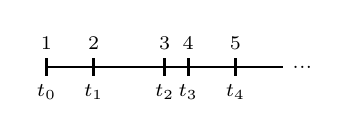
\begin{tikzpicture}[
    sync/.style={fill,inner xsep=0pt},
    decoration={
      markings,
      mark=at position .0 with {\mksynch{$t_0$}{$1$}},
      mark=at position .2 with {\mksynch{$t_1$}{$2$}},
      mark=at position .5 with {\mksynch{$t_2$}{$3$}},
      mark=at position .6 with {\mksynch{$t_3$}{$4$}},
      mark=at position .8 with {\mksynch{$t_4$}{$5$}},
      mark=at position 1 with {\node[anchor=west] {\scriptsize $...$};},
    }
    ]
    \draw[postaction=decorate, ] (0,0) -- (3,0); 
  \end{tikzpicture}
}
\newsavebox{\outsignal}
\savebox{\outsignal}{
  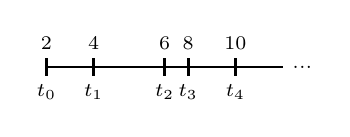
\begin{tikzpicture}[
    sync/.style={fill,inner xsep=0pt},
    decoration={
      markings,
      mark=at position .0 with {\mksynch{$t_0$}{$2$}},
      mark=at position .2 with {\mksynch{$t_1$}{$4$}},
      mark=at position .5 with {\mksynch{$t_2$}{$6$}},
      mark=at position .6 with {\mksynch{$t_3$}{$8$}},
      mark=at position .8 with {\mksynch{$t_4$}{$10$}},
      mark=at position 1 with {\node[anchor=west] {\scriptsize $...$};},
    }
    ]
    \draw[postaction=decorate, ] (0,0) -- (3,0); 
  \end{tikzpicture}
}

\begin{docimage}{example}
\begin{tikzpicture}
  \standard[process, moc=sy, ni=2, no=1, nf=1, f1=$(+)$, type=comb](p1){P};
  \node (t1) at ($(p1.w1)-(3,-.5)$) {\usebox{\insignal}};
  \node (t2) at ($(p1.w2)-(3,.5)$) {\usebox{\insignal}}; 
  \node (t3) at ($(p1.e1)+(3,0)$) {\usebox{\outsignal}}; 
 
  \signal[-|-] (t1.east) -> (p1.w1); 
  \signal[-|-] (t2.east) -> (p1.w2);
  \signal[   ] (p1.e1) -> (t3.west);
\end{tikzpicture}
\end{docimage}   

\begin{docimage}{pattern-delay}
\begin{tikzpicture}[]
  \standard[process, moc=sy, f=$0$, type=delay](p1){};
  \inputSY*  <p1.west> {1,2,3,4,5};
  \outputSY* <p1.east> {0,1,2,3,4,5};
\end{tikzpicture}
\end{docimage} 

\begin{docimage}{pattern-comb}
\begin{tikzpicture}[]
  \standard[process, moc=sy, ni=2, no=2, f={$\lambda\ a\ b \rightarrow (a+b,a-b)$}, type=comb](p1){};
  \inputSY*[anchor=south west, shift={(-2cm, .2cm)}]  <p1.w1> {1,2,3,4,5,6,...};
  \inputSY*[anchor=south west, shift={(-2cm,-.2cm)}]  <p1.w2> {1,1,1,1,1};
  \outputSY*[yshift=.2cm]  <p1.e1> {2,3,4,5,6};
  \outputSY*[yshift=-.2cm]  <p1.e2> {0,1,2,3,4};
\end{tikzpicture}
\end{docimage} 

\begin{docimage}{pattern-reconfig}
\begin{tikzpicture}[]
  \standard[process, moc=sy, ni=2, no=1, type=reconfig](p1){};
  \inputSY*[anchor=south west, shift={(-4cm, .2cm)}]  <p1.w1> {$+1,\times 2,+1,\times 2,+1,\times 2,+1$};
  \inputSY*[anchor=south west, shift={(-4cm,-.2cm)}]  <p1.w2> {$1,2,3,4,5,6,7,8,...$};
  \outputSY*  <p1.e1> {$2,4,4,8,6,12,8$};
\end{tikzpicture}
\end{docimage} 

\begin{docimage}{pattern-constant}
\begin{tikzpicture}[]
  \standard[process, moc=sy, no=2, f={$(1,2)$}, type=constant](p1){};
  \outputSY*[yshift=.2cm]  <p1.e1> {$1,1,1,...$};
  \outputSY*[yshift=-.2cm] <p1.e2> {$2,2,2,...$};
\end{tikzpicture}
\end{docimage} 

\begin{docimage}{pattern-generate}
\begin{tikzpicture}[]
  \standard[process, moc=sy, no=2, f={$\lambda\ a\ b \rightarrow (a+1,b+2)$}, type=generate](p1){};
  \outputSY*[yshift=.2cm]  <p1.e1> {$1,2,3,4,5,...$};
  \outputSY*[yshift=-.2cm] <p1.e2> {$2,4,6,8,10,...$};
\end{tikzpicture}
\end{docimage} 

\begin{docimage}{pattern-state}
\begin{tikzpicture}[]
  \standard[process, moc=sy, f={$+$;1}, type=state](p1){};
  \inputSY*  <p1.west> {1,2,3,4,5};
  \outputSY* <p1.east> {2,4,7,11,16};
\end{tikzpicture}
\end{docimage} 

\begin{docimage}{pattern-stated}
\begin{tikzpicture}[]
  \standard[process, moc=sy, f={$+$;1}, type=stated](p1){};
  \inputSY*  <p1.west> {1,2,3,4,5};
  \outputSY* <p1.east> {1,2,4,7,11,16};
\end{tikzpicture}
\end{docimage}

\begin{docimage}{pattern-moore}
\begin{tikzpicture}[]
  \standard[process, moc=sy, f={$+$;$+1$;1}, type=moore](p1){};
  \inputSY*  <p1.west> {1,2,3,4,5};
  \outputSY* <p1.east> {2,3,5,8,12,17};
\end{tikzpicture}
\end{docimage}

\begin{docimage}{pattern-mealy}
\begin{tikzpicture}[]
  \standard[process, moc=sy, f={$+$;$-$;1}, type=mealy](p1){};
  \inputSY*  <p1.west> {1,2,3,4,5};
  \outputSY* <p1.east> {0,0,1,3,6};
\end{tikzpicture}
\end{docimage}

\begin{docimage}{pattern-when}
\begin{tikzpicture}[]
  \standard[process, moc=sy, ni=2, no=1, type=when](p1){};
  \inputSY*[anchor=south west, shift={(-3cm, .2cm)}]  <p1.w1> {$F,F,F,T,T,...$};
  \inputSY*[anchor=south west, shift={(-3cm,-.2cm)}]  <p1.w2> {$1,2,3,4,5,...$};
  \outputSY*  <p1.e1> {$\bot,\bot,\bot,4,5,...$};
\end{tikzpicture}
\end{docimage} 

\begin{docimage}{pattern-filter}
\begin{tikzpicture}[]
  \standard[process, moc=sy, f={$>3$}, type=filter](p1){};
  \inputSY*  <p1.west> {$1,2,3,4,5,...$};
  \outputSY* <p1.east> {$\bot,\bot,\bot,4,5,...$};
\end{tikzpicture}
\end{docimage}

\begin{docimage}{pattern-fill}
\begin{tikzpicture}[]
  \standard[process, moc=sy, f={$0$}, type=fill](p1){};
  \inputSY*  <p1.west> {$\bot,\bot,1,2,\bot,3$};
  \outputSY* <p1.east> {$0,0,1,2,0,3$};
\end{tikzpicture}
\end{docimage}

\begin{docimage}{pattern-hold}
\begin{tikzpicture}[]
  \standard[process, moc=sy, f={$0$}, type=hold](p1){};
  \inputSY*  <p1.west> {$\bot,\bot,1,2,\bot,3$};
  \outputSY* <p1.east> {$0,0,1,2,2,3$};
\end{tikzpicture}
\end{docimage}

\begin{docimage}{pattern-reactAbst}
\begin{tikzpicture}[]
  \standard[process, moc=sy, f={$\noexpand\BhCons{ignore}(+)$;$0$}, type=stated](p1){};
  \cluster[process, inner sep=16pt, moc=sy, type=reactAbst] <(p1)> {};
  \inputSY*  <p1.west> {$1,1,1,\bot,1,\bot,1$};
  \outputSY* <p1.east> {$0,1,2,\bot,3,\bot,4$};
\end{tikzpicture}
\end{docimage}

\begin{docimage}{tode}%
\begin{tikzpicture}[]
  \standard[process, ni=2, moc=sy, type=toDE](p1){};
  \inputSY*[yshift=.2cm]  <p1.w1> {$0,3,4,6,9$};
  \inputSY*[yshift=-.2cm]  <p1.w2> {$1,2,3,4,5$};
  \begin{signalsDE}[grid and time=5,outputs={p1}, xscale=.4]{10}
    \signalDE{ 1:0, 2:3, 3:4, 4:6, 5:9, 5:30 }
  \end{signalsDE}
\end{tikzpicture}
\end{docimage}

\begin{docimage}{tosdf}
\begin{tikzpicture}
  \standard[process, moc=sy, type=toSDF](p1){};
  \inputSY*  <p1.w1> {1,2,3,4,5};
  \outputSY* <p1.e1> {1,2,3,4,5};
\end{tikzpicture}
\end{docimage}

\begin{docimage}{tosdfp}
\begin{tikzpicture}[]
  \standard[process, ni=1, moc=sdf, type=toSDF'](p1){};
  \node[anchor=south east, xshift=-1cm] (p1w1) at (p1.w1) {%
    $\begin{array}{cccc}
      \vbvec & \vbvec & \vbvec & \vbvec \\
      1  & 3  & 5  & 7  \\
      2  & 4  & 6  & 8  \\
      \vevec & \vevec & \vevec & \vevec
    \end{array}$
  };
  \outputSY*  <p1.e1> {1,2,3,4,5,6,7,8};
  \path[s,<-] (p1.e1) edge (p1w1.south west);
  \resetportinfo{p1}\wpinfo{2}
\end{tikzpicture}
\end{docimage}


\begin{docimage}{zipx}
\begin{tikzpicture}[]\scriptsize
  \trans[transition=s1v1, rotate shape=180, ni=4, moc=sdf, type=zipx](p1){};
  \node[shift={(-3, .35)}, anchor=south west] (p1w1) at (p1.w1) {1,2,3,4,5};
  \node[shift={(-3, .15)}, anchor=south west] (p1w2) at (p1.w2) {1,2,3,4,5};
  \node[shift={(-3,-.15)}, anchor=south west] (p1w3) at (p1.w3) {11,12,13,14,15};
  \node[shift={(-3,-.35)}, anchor=south west] (p1w4) at (p1.w4) {11,12,13,14,15};
  \node[anchor=south west, xshift=1cm] (p1e1) at (p1.e1) {%
    $\begin{array}{ccccc}
      \vbvec & \vbvec & \vbvec & \vbvec & \vbvec \\
      1  & 2 & 3 & 4 & 5 \\
      1  & 2 & 3 & 4 & 5 \\
      11 & 12 & 13 & 14 & 15 \\
      11 & 12 & 13 & 14 & 15 \\
      \vevec & \vevec & \vevec & \vevec & \vevec
    \end{array}$
  };
  \path[s,->, -|-=.9]
  (p1w1.south west) edge (p1.w1)
  (p1w2.south west) edge (p1.w2)
  (p1w3.south west) edge (p1.w3)
  (p1w4.south west) edge (p1.w4)
  (p1.e1) edge (p1e1.south east);
\end{tikzpicture}
\end{docimage}

\begin{docimage}{unzipx}
\begin{tikzpicture}[]\scriptsize
  \trans[transition=s1v1, no=4, moc=sdf, type=zipx](p1){};
  \node[shift={(3, .35)}, anchor=south east] (p1e1) at (p1.e1) {1,1,1,1,1};
  \node[shift={(3, .15)}, anchor=south east] (p1e2) at (p1.e2) {2,2,2,2,2};
  \node[shift={(3,-.15)}, anchor=south east] (p1e3) at (p1.e3) {3,3,3,3,3};
  \node[shift={(3,-.35)}, anchor=south east] (p1e4) at (p1.e4) {4,4,4,4,4};
  \node[anchor=south east, xshift=-1cm] (p1w1) at (p1.w1) {%
    $\begin{array}{ccccc}
      \vbvec & \vbvec & \vbvec & \vbvec & \vbvec \\
      1  & 1 & 1 & 1 & 1 \\
      2  & 2 & 2 & 2 & 2 \\
      3  & 3 & 3 & 3 & 3 \\
      4  & 4 & 4 & 4 & 4 \\
      \vevec & \vevec & \vevec & \vevec & \vevec
    \end{array}$
  };
  \path[s,<-, -|-=.9]
  (p1e1.south east) edge (p1.e1)
  (p1e2.south east) edge (p1.e2)
  (p1e3.south east) edge (p1.e3)
  (p1e4.south east) edge (p1.e4)
  (p1.w1) edge (p1w1.south west);
\end{tikzpicture}
\end{docimage}



\end{document}

%%% Local Variables:
%%% TeX-command-default: "Make"
%%% mode: latex
%%% TeX-master: t
%%% End:
